% makeindex < aebpro_man.idx > aebpro_man.ind
\documentclass{article}
\usepackage[fleqn]{amsmath}
\usepackage[
    web={centertitlepage,designv,forcolorpaper,latextoc,pro},
    eforms,
    linktoattachments,
    aebxmp
]{aeb_pro}
\usepackage{graphicx,array}
%\usepackage{myriadpro}
%\usepackage{calibri}
\usepackage[altbullet]{lucidbry}

%\usepackage{makeidx}
%\makeindex
\usepackage{acroman}
\usepackage[active]{srcltx}

%\urlstyle{rm}
\urlstyle{sf}

\DeclareDocInfo
{
    university={NORTHWEST FLORIDA STATE COLLEGE\\
        Department of Mathematics},
    title={eCards: Electronic Flash Cards\texorpdfstring{\\[3ex]}{,} Manual of Usage},
    author={D. P. Story},
    email={dpstory@acrotex.net},
    subject={Documentation for the eCards package from AcroTeX},
    talksite={\url{www.acrotex.net}},
    version={2.0, 2016/09/03},
    keywords={AcroTeX, flash cards, interactive},
    copyrightStatus=True,
    copyrightNotice={Copyright (C) \the\year, D. P. Story},
    copyrightInfoURL={http://www.acrotex.net}
}

\def\dps{$\hbox{$\mathfrak D$\kern-.3em\hbox{$\mathfrak P$}%
   \kern-.6em \hbox{$\mathcal S$}}$}

\universityLayout{fontsize=Large}
\titleLayout{fontsize=LARGE}
\authorLayout{fontsize=Large}
\tocLayout{fontsize=Large,color=aeb}
\sectionLayout{indent=-62.5pt,fontsize=large,color=aeb}
\subsectionLayout{indent=-31.25pt,color=aeb}
\subsubsectionLayout{indent=0pt,color=aeb}
\subsubDefaultDing{\texorpdfstring{$\bullet$}{\textrm\textbullet}}

\widestNumber{0.00.}
%\pagestyle{empty}
%\parindent0pt\parskip\medskipamount

\def\dps{$\mbox{$\mathfrak D$\kern-.3em\mbox{$\mathfrak P$}%
   \kern-.6em \hbox{$\mathcal S$}}$}

\frenchspacing

\chngDocObjectTo{\newDO}{doc}
\begin{docassembly}
var titleOfManual="The AeB eCards MANUAL";
var manualfilename="Manual_BG_Print_ecards.pdf";
var manualtemplate="Manual_BG_Green.pdf"; // Blue, Green, Brown
var _pathToBlank="C:/Users/Public/Documents/ManualBGs/"+manualtemplate;
var doc;
var buildIt=true;
if ( buildIt ) {
    console.println("Creating new " + manualfilename + " file.");
    doc = \appopenDoc({cPath: _pathToBlank, bHidden: true});
    var _path=this.path;
    var pos=_path.lastIndexOf("/");
    _path=_path.substring(0,pos)+"/"+manualfilename;
    \docSaveAs\newDO ({ cPath: _path });
    doc.closeDoc();
    doc = \appopenDoc({cPath: manualfilename, oDoc:this, bHidden: true});
    f=doc.getField("ManualTitle");
    f.value=titleOfManual;
    doc.flattenPages();
    \docSaveAs\newDO({ cPath: manualfilename });
    doc.closeDoc();
} else {
    console.println("Using the current "+manualfilename+" file.");
}
var _path=this.path;
var pos=_path.lastIndexOf("/");
_path=_path.substring(0,pos)+"/"+manualfilename;
\addWatermarkFromFile({
    bOnTop:false,
    bOnPrint:false,
    cDIPath:_path
});
\executeSave();
\end{docassembly}

\begin{document}

\maketitle

\selectColors{linkColor=black}
\tableofcontents
\selectColors{linkColor=webgreen}


%--------------
%\usepackage{amsmath}
%\usepackage[designi,dvipsone,tight,latextoc,nodirectory,usesf]{web}
%%\usepackage[dvipsone,designi,latextoc,forpaper,nodirectory,usesf]{web}
%%\usepackage[nocorrections]{exerquiz}
%\usepackage{verbatim}
%% \usepackage{longtable,colortbl}
%% \usepackage{pifont}
%\usepackage[usecmtt]{myriadpro}



%\pdfstringdefDisableCommands{\let\!\empty}

% \setlongtables

\def\AcroT{Acro\!\TeX}\def\cAcroT{\textcolor{blue}{\AcroT}}
\def\AcroEB{\AcroT{} eDucation Bundle}\def\cAcroEB{\textcolor{blue}{\AcroEB}}
\def\AcroB{\AcroT{} Bundle}\def\cAcroB{\textcolor{blue}{\AcroB}}
\def\bUrl{http://www.math.uakron.edu/~dpstory}

\hypersetup{linktocpage}

%\newenvironment{sverbatim}
%{\par\footnotesize\verbatim}{\endverbatim\noindent}
%
%\newcommand\redpoint{\par\ifdim\lastskip>0pt\relax\vskip-\lastskip\fi
%\vskip\medskipamount\noindent
%  \makebox[\parindent][l]{\large\color{red}$\blacktriangleright$}}
%\newcommand\handpoint{\par\ifdim\lastskip>0pt\relax\vskip-\lastskip\fi
%\vskip\medskipamount\noindent
%  \makebox[\parindent][l]{\large\color{blue}\ding{042}}}

%\newcommand{\cs}[1]{\texttt{\char`\\#1}}


%\begin{document}
%
%\maketitle
%\tableofcontents

\section{Introduction}

The initial version of this package was developed at the request of my colleague, Dr.\ Thomas
Price for use in the senior honors project of Ms.\ Katie Jones on
\href{http://www.math.uakron.edu/~teprice/Trig/}{Trig Flash Cards}.
Upon completion of the honors project, I generalized and extended
the original package developed specifically for them.

Version~2.0 (2016/07/20) of \app{eCards} brings the package up to date with
the \pkg{exerquiz} package, which has undergone considerable revision since
\app{eCards} first appeared. The only changes in the package is its name, the
package name is \texttt{ecards} rather than \app{eCards}, also,
\pkg{exerquiz} package dated 2016/04/18 or later is required.

\section{Overview}

We give a graphical overview of \app{eCards} using the demonstration file
\texttt{ecardstst.tex}. There are three types of pages, excluding the cover
page: the question page, the hint page, and the answer page.

\begin{figure}[htb]
\hskip-62.5pt\begin{minipage}{\linewidth+62.5pt}
\centering
\includegraphics[width=.32\linewidth]{graphics/ecardstst-panel-ques}\hfill
\includegraphics[width=.32\linewidth]{graphics/ecardstst-panel-hint}\hfill
\includegraphics[width=.32\linewidth]{graphics/ecardstst-panel-ans}\hfill
  \caption{The question, hint, and answer pages with panel}\label{fig:ecards-pan}
\end{minipage}
\end{figure}

\hyperref[fig:ecards-pan]{Figure~\ref*{fig:ecards-pan}} shows the demonstration document using the
\opt{rightpanel} option; the user navigates through the document by pressing
the links labeled `Hint', `Soln', `Next', and `Prev'.

Using the \opt{usetemplates} option instead of \opt{rightpanel} renders the
same pages as shown in \hyperref[fig:ecards-nopan]{Figure~\ref*{fig:ecards-nopan}}.

\begin{figure}[htb]
\hskip-62.5pt\begin{minipage}{\linewidth+62.5pt}
\centering
\includegraphics[width=.32\linewidth]{graphics/ecardstst-nopanel-ques}\hfill
\includegraphics[width=.32\linewidth]{graphics/ecardstst-nopanel-hint}\hfill
\includegraphics[width=.32\linewidth]{graphics/ecardstst-nopanel-ans}\hfill
  \caption{The question, hint, and answer pages with no panel}\label{fig:ecards-nopan}
\end{minipage}
\end{figure}

In the case of \opt{usetemplates},
\hyperref[fig:ecards-nopan]{Figure~\ref*{fig:ecards-nopan}}, the user works
through the cards using the navigation icons in to footer of the page.

When the \opt{listing} option is used along with the \opt{forpaper} option, a
document suitable for printing is produced. The document contains the
questions, hints, and solutions for the document author to conveniently
review. This document is shown in \hyperref[fig:ecards-listing]{Figure~\ref*{fig:ecards-listing}}.

\begin{figure}[htb]\centering\setlength{\fboxsep}{0pt}\fbox
{\includegraphics[width=.67\linewidth]{graphics/ecardstst-listing}}
  \caption{The cards with the \texttt{listing} option}\label{fig:ecards-listing}
\end{figure}

\section{Documentation}

In this section, the major elements of this package are highlighted. For those
who want to know more, you can peruse the {\LaTeX} code, there are comments
contained there as well.  The document \texttt{ecardstst.tex} illustrates
most of what you need to know for creating your own electronic flash cards.

\subsection{Preamble: Required packages and options}

\subsubsection{Required packages}

This package depends heavily on the
\textbf{\href{http://www.math.uakron.edu/~dpstory/webeq.html}
{Acro\negthinspace\TeX{} eDucation Bundle}}: (1) the \pkg{web} package
provides page setup, backgrounds, and navigational elements; (2) the
\pkg{exerquiz} package (dated 2016/04/18 or later) allows you to author the
questions, both non-responsive and responsive (fill-in and multiple choice);
and (3) the \pkg{insdljs} packages is the mechanism for introducing
document-level JavaScripts into the final document.

\subsubsection{Drivers}

The supported drivers are the same as those supported by \pkg{exerquiz}:
\texttt{dvipsone}, \texttt{dvips}, \texttt{pdftex}, and \texttt{xetex}.

A typical set of packages used for on screen presentation:
\begin{Verbatim}[xleftmargin=\amtIndent,commandchars=!()]
\usepackage[!ameta(driver_option),tight,rightpanel]{web}
\usepackage[!ameta(options)]{exerquiz}
\usepackage[!ameta(options)]{ecards}
\end{Verbatim}
where \ameta{driver\_option} is any of the drivers listed above;
\texttt{pdftex} and \texttt{xetex} are automatically detected so they need
not be specified; if the driver option \texttt{dvips} is specified in the
\texttt{web.cfg},  it need not be specified either.

\paragraph*{A note on \app{xetex}.}
The \app{xetex} application may be set to strip out named destinations that
are not referenced within the document as a target of a `hard-wired' link.
The \pkg{ecards} package sets a lot of destinations (or targets) but, in many
instances, `dynamic' links are employed using the JavaScript method
\texttt{\textsl{Doc}.gotoNamedDest(\ameta{target})}. In such instances,
\app{xetex} may strip out these targets; the link or button action may not
perform the jump to the destination because the destination does not exist.
If this becomes an issue for your \app{xetex} installation, the
\textbf{\app{Dvipdfmx} Compatibility Flags} needs to be modified. Search for
the configuration file \texttt{dvipdfmx.cfg}, open the file. Scroll down to
the line `\texttt{\%C  0x0000}', beneath it insert `\texttt{C  0x0010}', save
and close the file.\footnote{MiK\TeX{} discourages the direct editing of the
file \texttt{dvipdfmx.cfg}, instead, on the command-line prompt type and
execute `\texttt{initexmf -{}-edit-config-file dvipdfmx}' enabling you to edit
a local version of the configuration file as described above.} The
documentation for this bit field is just above the referenced line and an
explanation of the `\texttt{C 0x0010}' setting is given.


\subsubsection{Options}

\paragraph*{\app{eCards} options.}\hskip-\lastskip\
The \pkg{ecards} package really has only 4 options:
\begin{enumerate}
   \item \texttt{nohints}: If you do not want to provide hints in your \app{eCards},
       use this option. See also the comments in \Nameref{hint}.

     The default is to provide and display hints to each card; when
     \opt{nohints} is specified in the option list of \pkg{ecards}, no
     hints provided becomes the default.

     Whether hints are provided or not can be overridden in two ways:
     through the optional argument of the \env{card} environment
     (\autopageref{ss:cardEnv}), and through the commands listed next.
\bVerb\takeMeasure{\string\useNoHints\quad\string\useHints}%
\begin{dCmd}[commandchars=!()]{\bxSize}
\useNoHints!quad\useHints
\end{dCmd}
\eVerb The commands are used between \env{card} environments to change the
default usage of hints. When hints are \emph{not provided}, a simple message
defined by the command \cs{noHintProvided} (see \autopageref{noHintProvided}) appears on the hint page.

   \item \texttt{listing}:\label{listing} This option gives you a printable version of your
       \app{eCards}. In this way, you can proofread, check your questions, hints,
       and answers. Suggested packages and options are given below:
\begin{Verbatim}[xleftmargin=\amtIndent,commandchars=!()]
\usepackage[!ameta(driver_option),forpaper]{web}
\usepackage[solutionsafter,proofing]{exerquiz}
\usepackage[listing]{ecards}
\end{Verbatim}
This option sets the Boolean \cs{ifecListing} to true; this Boolean is used
to define optional content. Read \Nameref{ss:cardEnv} for an example of
using \cs{ifecListing}.

Refer to \hyperref[fig:ecards-listing]{Figure~\ref*{fig:ecards-listing}}
  for a depiction of an \app{eCards} document under the \opt{listing}
  option.
  \item \texttt{memLogo}: The logo, if any, is read and re-read
      for each page on which it appears.  Using this option, the logo
   is read once and saved in a box for use.
  \item \texttt{custom}: If this option is included in the option list, the
      package looks for and inputs the file \texttt{ecard.cus}. This file
      can be used to customize the environments. This file should be kept
      in the source directory, not in the {\LaTeX} search path.
\end{enumerate}

\paragraph*{Other options.}
Selecting the various options of the \textsf{web} and
\textsf{exerquiz} packages can give you different looks.  It is
important to be aware of all the options associated with these
two package; in the paragraphs below, various options are
discussed that may be useful in \app{eCards}.

\subparagraph*{Useful \pkg{web} package options.}
There are three background/\penalty0panel options; these are \texttt{usetemplates},
\texttt{rightpanel} and \texttt{leftpanel}.

Using the \texttt{usetemplates} option does not give you the vertical
navigation panel, but it does provide background colors; the
\texttt{rightpanel} and \texttt{leftpanel} given you a vertical panel on the
right and left, respectively.  Use one of these three options only, if any at
all. Using none of these three will just get you the default white
background. See the {\AEB} documentation for details.

There are certain ``standard'' page designs, or you can create your own using
the \cs{margins} and \cs{screensize}; the demo document has
\begin{Verbatim}
    \margins{.25in}{.25in}{24pt}{.25in} % left,right,top, bottom
    \screensize{3.72in}{366.24bp}       % height, width
\end{Verbatim}
See the \pkg{web} package documentation for details on these and other
options.

\subparagraph*{Useful \pkg{exerquiz} package options.}
If you are not using  multiple choice or fill-in questions, you should use
the \texttt{exercisesonly} option. This removes much of the document level JavaScript
from the PDF document.

For authors that use the full Acrobat~5.0, or the newer Acrobat
6.0 Standard or Acrobat 6.0 Professional, you can use the
\texttt{execJS} option. If this option is taken, then when the
document is first loaded into Acrobat (following distillation, or
creation using \textsf{dvipdfm} or \textsf{pdftex}), the document
will be automatically saved; this saves any imported document
level JavaScript in the document. The document always needs to be saved
after creation so save the scripts with the document, this does it automatically
so you can't forget to do it---as one of my colleagues once did.

The \texttt{nosolutions} option removes the \texttt{response} environment
leaving only the questions. The \texttt{proofing} and \texttt{preview} options
can be useful for proofreading, as described in the \texttt{\hyperref[listing]{listing}}
option described above.

\subsubsection{Original customization commands}\label{ss:origCus}

The \app{eCards} defines several (text) commands, there are listed here:
\begin{itemize}
\item \cs{cardsFinishedMsg}: When the user has reviewed all the electronic flash cards,
    an alert dialog appears with a message. The contents of the message are defined by
    this command. The default is
\begin{Verbatim}[xleftmargin=\amtIndent]
\cardsFinishedMsg{You've seen all the cards!}
\end{Verbatim}

\item \cs{cardColor}, \cs{hintColor}, and \cs{solnColor}: The background colors of various pages.
The defaults are
\begin{Verbatim}[xleftmargin=\amtIndent]
\cardColor{vlightblue}
\hintColor{cornsilk}
\solnColor{webyellow}
\end{Verbatim}
Additionally, \cs{textBgColor} command is used to define the default
background color (of the \pkg{web} package). This will be the color of the
first page, the default is \cs{textBgColor\darg{cornsilk}}. The panel
background is controlled by the \pkg{web} command \cs{panelBgColor}; for
example, \cs{panelBgColor\darg{logoblue}}.

\item \cs{ecLogo}: The logo emblem that would appear in the upper portion of the vertical
    navigational strip. This assumes  you are using either the \texttt{rightpanel} or
    \texttt{leftpanel} option for \textsf{web}. The default is
\begin{Verbatim}[xleftmargin=\amtIndent]
\ecLogo{\includegraphics[scale=.4]{graphics/uakron}}
\end{Verbatim}
As you can see, the argument of this command is a graphic command, usually the command
\cs{includegraphics} from the \textsf{graphicx} package.

\item \cs{ecLogoLink}: This is the URL of the link destination that will be placed
    around the logo. The default is an empty address, in this case, no link is placed
    around the logo emblem. An example of usage:
\begin{Verbatim}[xleftmargin=\amtIndent]
\ecLogoLink{http://www.uakron.edu/}
\end{Verbatim}

\item \cs{ecHomePage}: This is the URL to a page. This will be used as a link destination
    of the `Home' button seen on the first page of the \app{eCards} document.
\begin{Verbatim}[xleftmargin=\amtIndent,fontsize=\small]
\ecHomePage{http://www.math.uakron.edu/~dpstory/acrotex.html}
\end{Verbatim}

\item \cs{noHintJSAction}: When there are no hints (the document author has taken the
option \texttt{nohints}, the `hints' button is grayed out, but still functional, with
no JavaScript action. You can add some action to this button through this command.
An example of usage is
\begin{Verbatim}[xleftmargin=\amtIndent,fontsize=\small]
\renewcommand\noHintJSAction{app.alert("No hints provided!")}
\end{Verbatim}
\end{itemize}
\hyperref[s:addiCus]{Section~\ref*{s:addiCus}} lists more customization
commands, available with version~2 or later of \app{eCards}.

\subsection{\texorpdfstring{\protect\cs{begin\{document\}}}
{\textbackslash{begin\{document\}}}: Start creating cards}

The process of creating these electronic cards is quite simple, the sections below
describe the \texttt{card}, \texttt{response}, \texttt{hint} and \texttt{answers} environments.

\subsubsection{The \texttt{card} environment}\label{ss:cardEnv}

The main environment is the \texttt{card} environment, which is used for posing
questions, offering a hint, and an answer. The \hypertarget{cardsyntax}{syntax} is,
\bVerb\takeMeasure{\string\begin\darg{card}[hint|nohint]}%
\begin{dCmd}[commandchars=!()]{\bxSize}
\begin{card}[hint|nohint]
  !ameta(a question)
  \begin{response}
      \begin{hint}
      !ameta(a hint)
      \end{hint}
      \begin{answer}
      !ameta(an answer)
      \end{answer}
  \end{response}
\end{card}
\end{dCmd}
\eVerb The optional parameter takes one of two keys,
\texttt{hint} or \texttt{nohint}. Normally, each question contains a hint,
but there is an option, \texttt{nohints}, for declaring that no hints are to
be used for the question. You can pass one of these two parameters into the
\texttt{card} environment to declare there is a hint for this question (in
the case \texttt{nohints} is selected as an option), or to declare there is
no hint for this question (in the case \texttt{nohints} \emph{is not} an
option).  If no parameter is passed, it is assumed the question has a hint,
unless the \texttt{nohints} option is used, in which case it is assumed the
question has no  hint.

Below is the first \env{card} environment for \texttt{ecardstst.tex} showing the nesting
of the \env{card}, \env{response}, \env{hint}, and \env{answer} environments.
\begin{Verbatim}[xleftmargin=\amtIndent,fontsize=\small]
\begin{card}
    Who was the first President of the United States?
\begin{response}
    \begin{hint}
        Legend has it, he chopped down the cherry tree and
        couldn't tell a lie.
    \end{hint}
    \begin{answer}
    \ifecListing
        George Washington (1789-1797)
    \else\centering
        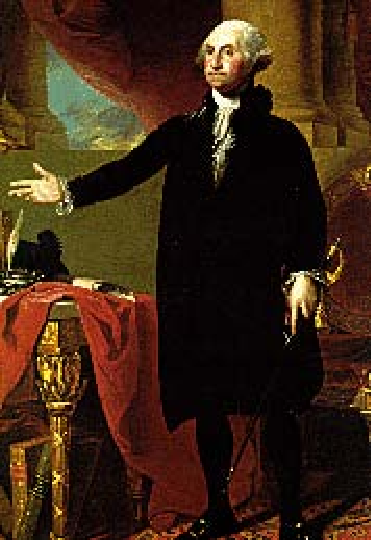
\includegraphics[scale=.4]{presidents/gw1}\\
            George Washington\\
            1789-1797
    \fi
    \end{answer}
\end{response}
\end{card}
\end{Verbatim}
The role of \cs{ifecListing} is also shown in the above verbatim listing.
When \opt{listing} is specified, there is no need for the graphic; we use a
text phrase instead.


\newtopic\noindent\textbf{\textcolor{red}{Important.}} You can pose a question which requires
a verbal response, or one for which there is a choice of
alternatives, or a fill-in the blank (math or text). See the demo
file \texttt{ecardstst.tex} for examples.

\subsubsection{The \texttt{response} environment}

Immediately following and nesting within the \env{card} environment is the
\env{response} environment.  This sets things up for the responses to the
question: the hint and the answer.

\subsubsection{The \texttt{hint} environment}\label{hint}

The first environment to appear within the \texttt{response} is
the \env{hint} environment.  Here you can provide additional
information to help the student answer the question successfully.
I've posed a multiple choice or fill-in question, you can simply
copy the multiple choice or fill-in into the hint, just as I have done
in the demo file \texttt{ecardstst.tex}.

In this release, hints can be provided for \textbf{all} of the questions or
for \textbf{none} of the questions. You can enter hints using the \env{hint}
environment, illustrated \hyperlink{cardsyntax}{above}, or not include a
\env{hint} environment.  When you do not want to include hints---whether
you've entered the environments or not---use the \opt{nohints} package
option. This will convert the \env{hint} environment into a \texttt{comments}
environment, and redefine some of the navigational buttons.

\subsubsection{The \texttt{answer} environment}

After the \env{hint} environment comes the answer environment where the answer to
the original question can be presented. At the end of this environment, you
need to back out of the nested environments: \cs{end\darg{answer}},
\cs{end\darg{response}} and \cs{end\darg{card}}.

\subsection{\texorpdfstring{\protect\cs{end\{document\}}}{\textbackslash{end\{document\}}}}

That's the end!  Once you have completed your \app{eCards} file, you are
ready to create your \app{eCards} PDF document!
%The \app{eCards} package supports PDF
%creation using any of the following methods:
%\begin{enumerate}
%    \item  $\text{\texttt{.tex}}\mapsto\text{\texttt{.dvi}}\mapsto\text{\texttt{.ps}}\mapsto\text{\texttt{.pdf}}$.
%    This route uses the \texttt{dvipsone} or \texttt{dvips} option
%    (for the \textsf{web} package), followed by the use of the
%    Acrobat Distiller (Version 5.0 or later suggested).
%    \item $\text{\texttt{.tex}}\mapsto\text{\texttt{.dvi}}\mapsto\text{\texttt{.pdf}}$. Here, you latex the
%    document, then hit the result using \textsf{dvipdfm}. Naturally, you would use the \texttt{dvipdfm}
%    option with the \textsf{web} package.
%    \item $\text{\texttt{.tex}}\mapsto\text{\texttt{.pdf}}$. Here, you use the \texttt{pdftex} option
%    of \textsf{web}, and \textsf{pdflatex} the document.
%\end{enumerate}


\subsection{Additional customization commands}\label{s:addiCus}

Version~2.0 or later has a number of commands designed to customize the look of \app{eCards} without
having to redefine some of the environments.

\subsubsection{The question page}

In addition to \cs{cardColor}, described briefly in \Nameref{ss:origCus}, the following are also defined
on the question page.
\bVerb\takeMeasure{\string\ecAfterQuesSkip\darg{\ameta{skip}}}%
\edef\x{\the\wd\webtempboxi}%
\def\1{\hbox to0pt{\hskip\x\relax\quad\normalfont(\texttt{.25in})\hss}}%
\def\2{\hbox to0pt{\hskip\x\relax\quad\normalfont(\texttt{.85\string\linewidth})\hss}}%
\takeMeasure{\string\renewcommand\darg{\string\ecQUESTION}\darg{\string\textbf\darg{QUESTION}}}%
\begin{dCmd}[commandchars=!()]{\bxSize}
\renewcommand{\ecQUESTION}{\textbf{QUESTION}}
!1\ecAfterQuesSkip{!ameta(skip)}
!2\ecQuesWidth{!ameta(length)}
\end{dCmd}
\eVerb The \cs{ecQUESTION} command defines the title for the question page;
the default definition is given. Beneath \cs{ecQUESTION} is a vertical space
of \ameta{skip} determined by the argument of \cs{ecAfterQuesSkip}, its
default is given in parenthesis. The content of the question page is
contained in a minipage of width \ameta{length} determined by the argument of
\cs{ecQuesWidth}, its default value is given in parenthesis.

\subsubsection{The hint page}

In addition to \cs{hintColor}, described briefly in \Nameref{ss:origCus}, the following are also defined
on the hint page.
\bVerb\takeMeasure{\string\ecAfterHintSkip\darg{\ameta{skip}}}%
\edef\x{\the\wd\webtempboxi}%
\def\1{\hbox to0pt{\hskip\x\relax\quad\normalfont(\texttt{.25in})\hss}}%
\def\2{\hbox to0pt{\hskip\x\relax\quad\normalfont(\texttt{.85\string\linewidth})\hss}}%
\takeMeasure{\string\ecAfterHintSkip\darg{\ameta{skip}}\quad\normalfont(\texttt{.85\string\linewidth})}%
\begin{dCmd}[commandchars=!()]{\bxSize}
\renewcommand{\ecHINT}{\textbf{HINT}}
!1\ecAfterHintSkip{!ameta(skip)}
!2\ecHintWidth{!ameta(length)}
\end{dCmd}
\eVerb The \cs{ecHINT} command defines the title for the hint page;
the default definition is given. Beneath \cs{ecHINT} is a vertical space
of \ameta{skip} determined by the argument of \cs{ecAfterHintSkip}, its
default is given in parenthesis. The content of the question page is
contained in a minipage of width \ameta{length} determined by the argument of
\cs{ecHintWidth}, its default value is given in parenthesis.



When there is no hint provided, the content of the \env{hint} environment is
not displayed, in its place the command \cs{noHintProvided} is expanded. The
default definition of which is given below.\phantomsection\label{noHintProvided}
\bVerb\takeMeasure{\string\renewcommand\darg{\string\noHintProvided}\darg{No hint provided for this question.}}%
\begin{dCmd}[commandchars=!()]{\bxSize}
\renewcommand{\noHintProvided}{No hint provided for this question.}
\end{dCmd}
\eVerb The command may be redefined as desired in the preamble.

\subsubsection{The answer page}

In addition to \cs{solnColor}, described briefly in \Nameref{ss:origCus}, the following are also defined
on the answer page.
\bVerb\takeMeasure{\string\ecAfterAnsSkip\darg{\ameta{skip}}}%
\edef\x{\the\wd\webtempboxi}%
\def\1{\hbox to0pt{\hskip\x\relax\quad\normalfont(\texttt{.25in})\hss}}%
\def\2{\hbox to0pt{\hskip\x\relax\quad\normalfont(\texttt{.85\string\linewidth})\hss}}%
\takeMeasure{\string\ecAfterAnsSkip\darg{\ameta{skip}}\quad\normalfont(\texttt{.85\string\linewidth})}%
\begin{dCmd}[commandchars=!()]{\bxSize}
\renewcommand{\ecANS}{\textbf{ANSWER}}
!1\ecAfterAnsSkip{!ameta(skip)}
!2\ecAnsWidth{!ameta(length)}
\end{dCmd}
\eVerb The \cs{ecANS} command defines the title for the answer page;
the default definition is given. Beneath \cs{ecANS} is a vertical space
of \ameta{skip} determined by the argument of \cs{ecAfterAnsSkip}, its
default is given in parenthesis. The content of the answer page is
contained in a minipage of width \ameta{length} determined by the argument of
\cs{ecAnsWidth}, its default value is given in parenthesis.

\subsubsection{The navigation icons}

The navigation icons have labels on them, which may be redefined for language
localization. The labels are defined through the arguments of the commands
below. The arguments given are the default (English) declarations.

\bVerb\takeMeasure{\string\ecHintSolnLabel\darg{Soln}    \string\ecRandomLabel\darg{Random}}%
\begin{dCmd}[commandchars=!()]{\bxSize}
\ecSolnLabel{Soln}        \ecBeginLabel{Begin}
\ecHintLabel{Hint}        \ecHomeLabel{Home}
\ecNextLabel{Next}        \ecFinHomeLabel{Home}
\ecPrevLabel{Prev}        \ecFSLabel{FS}
\ecHintNextLabel{Next}    \ecCloseLabel{Close}
\ecHintSolnLabel{Soln}    \ecRandomLabel{Random}
\end{dCmd}
\eVerb The meaning of these commands, it is hoped, is self-evident.

The size of the icons are determined by four commands.
\bVerb\takeMeasure{\string\renewcommand\string\iconWidthPanel\darg{28pt}}%
\begin{dCmd}[commandchars=!()]{\bxSize}
\renewcommand\iconWidth{40pt}
\renewcommand\iconHeight{15pt}
\renewcommand\iconWidthPanel{28pt}
\renewcommand\panelGrpWidth{57pt}
\end{dCmd}
\bVerb \cs{iconWidth} and \cs{iconHeight} set the dimensions of the
navigation icons when a panel option is not taken; \cs{iconWidthPanel} and
\cs{iconHeight} are the dimensions of the icons when they appear in the panel.
The \cs{panelGrpWidth} is the overall width of the group of icons in the
panel.

\subsubsection{The \texttt{listing} option}

There are some minor formatting commands that take effect when the
\opt{listing} option is used.
\bVerb\takeMeasure{\string\renewcommand\darg{\string\leadAnsFmtForPaper}\darg{\string\textbf\darg{Ans:\string\thinspace[}}}%
\begin{dCmd}[commandchars=!()]{\bxSize}
\renewcommand{\leadAnsFmtForPaper}{\textbf{Ans:\thinspace[}}
\renewcommand{\trailAnsFmtForPaper}{\textbf{]}}
\end{dCmd}
\bVerb The effects of this formatting is seen in
\hyperref[fig:ecards-listing]{Figure~\ref*{fig:ecards-listing}}; look for the bold
\texttt{Ans:} in question~4. To remove this formatting, simply redefine the
two commands
\begin{Verbatim}[xleftmargin=\amtIndent]
\renewcommand{\leadAnsFmtForPaper}{}
\renewcommand{\trailAnsFmtForPaper}{}
\end{Verbatim}
No formatting was the standard for \app{eCards} prior to version~2.0.

\subsubsection{Alert messages}

Several alert boxes appear in response to pressing buttons or links, we list
some of the more important ones. All redefinitions must occur in the preamble
of the document.
\bVerb\takeMeasure{\string\renewcommand\string\eqsqrtmsg\darg{"Right!"}}%
\begin{dCmd}[commandchars=*()]{\bxSize}
\renewcommand\eqsqrtmsg{"Right!"}
\renewcommand\eqsqwgmsg{"Wrong!"}
\end{dCmd}
\bVerb The above two definitions are from \pkg{exerquiz}, they are the message that appears (in an alert box)
to indicate to the user that his/her response is correct or wrong.

\bVerb\takeMeasure{\string\renewcommand\darg{\string\nonrandomizedMsg}\darg{The cards will be delivered}}%
\begin{dCmd}[commandchars=!()]{\bxSize}
\cardsFinishedMsg{You've seen all the cards!}
\renewcommand{\pressBeginMsg}{Press the \"Begin\" button to
    begin viewing the cards.}
\renewcommand{\randomizedMsg}{The cards will be delivered
    to you in random order.}
\renewcommand{\nonrandomizedMsg}{The cards will be delivered
    to you in their natural order.}
\end{dCmd}
\bVerb The first message appears when the user has gone through all the
cards. The second message appears when the user does not press the
``\textsf{Begin}'' button. The third and fourth inform the user the state of
the delivery of the cards; one of these messages appear when the state of the
``\textsf{Random}'' checkbox is changed.

\subsubsection{Miscellaneous customizations}

The ``\textsf{Random}'' checkbox has a tooltip message that can be
customized. Below is the default message.
\bVerb\takeMeasure{\string\renewcommand\darg{\string\toggleRandomizeTU}\{Click to toggle between}%
\begin{dCmd}[commandchars=!()]{\bxSize}
\renewcommand{\toggleRandomizeTU}{Click to toggle between
    random and natural order.}
\end{dCmd}
\bVerb

\subsubsection{\texorpdfstring{\protect\pkg{web}}{web} customizations}

The \pkg{web} package has may commands for modifying the look of the PDF page. The author is
referred to the {\AEB} manual for details.

%\revisionLabel and \versionLabel


\bigskip\noindent
Go to it, and be creative and enjoy! Now, back to my retirement. \dps

\end{document}

\bVerb\takeMeasure{\string\begin\darg{card}[hint|nohint]}%
\begin{dCmd}[commandchars=!()]{\bxSize}
\begin{card}[hint|nohint]
  !ameta(a question)
  \begin{response}
      \begin{hint}
      !ameta(a hint)
      \end{hint}
      \begin{answer}
      !ameta(an answer)
      \end{answer}
  \end{response}
\end{card}
\end{dCmd}
\eVerb
